%**************************************************************************
%* SpringSim 2020 Author Kit
%*
%* Word Processing System: TeXnicCenter and MiKTeX
%*
%**************************************************************************

\documentclass{scspaperproc}

\usepackage{latexsym}
\usepackage{graphicx}
\usepackage{mathptmx}

%
%****************************************************************************
% AUTHOR: You may want to use some of these packages. (Optional)
\usepackage{amsmath}
\usepackage{amsfonts}
\usepackage{amssymb}
\usepackage{amsbsy}
\usepackage{amsthm}
%****************************************************************************

%
%****************************************************************************
% AUTHOR: If you do not wish to use hyperlinks, then just comment
% out the hyperref usepackage commands below.

%% This version of the command is used if you use pdflatex. In this case you
%% cannot use ps or eps files for graphics, but pdf, jpeg, png etc are fine.

\usepackage[pdftex,colorlinks=true,urlcolor=blue,citecolor=black,anchorcolor=black,linkcolor=black,bookmarks=false]{hyperref}

%% The next versions of the hyperref command are used if you adopt the
%% outdated latex-dvips-ps2pdf route in generating your pdf file. In
%% this case you can use ps or eps files for graphics, but not pdf, jpeg, png etc.
%% However, the final pdf file should embed all fonts required which means that you have to use file
%% formats which can embed fonts. Please note that the final PDF file will not be generated on your computer!
%% If you are using WinEdt or PCTeX, then use the following. If you are using
%% Y&Y TeX then replace "dvips" with "dvipsone"

%% \usepackage[dvips,colorlinks=true,urlcolor=blue,citecolor=black,%
%% anchorcolor=black,linkcolor=black]{hyperref}

%% The use of the long citation format (e.g. "Brown and Edwards (1993)" rather than "[5]") and at the same
%% time using the hyperref package can lead to hard to trace bugs in case the citation is broken accross the
%% line (usually this will mark the entire paragraph as a hyperlink (clickable) which is easily noticeable and fixed
%% if using colorlinks, but not if the color is black -- as it is now). Worse yet, if a citation spans page boundary,
%% LaTeX compilation can fail, with an obscure error message. Since this depends a lot on the flow of the text
%% and wording, these bugs come and go and can be extremely hard for a beginner to trace. The error
%% message can look like this:
%%
%%    ! pdfTeX error (ext4): \pdfendlink ended up in different nesting level than \pdfstartlink.
%%    \AtBegShi@Output ...ipout \box \AtBeginShipoutBox 
%%    \fi \fi 
%%    l.174 
%%    ! ==> Fatal error occurred, no output PDF file produced!
%%
%% and can be universally fixed by putting an \mbox{} around the citation in question (in this case, at line 174)
%% and maybe adapting the wording a little bit to improve the paragraph typesetting, which is perhaps not
%% immediately obvious.
%****************************************************************************

%****************************************************************************
%*
%* AUTHOR: YOUR CALL!  Document-specific macros can come here.
%*
%****************************************************************************

%% ------ Package for adding bars into margin next to comments. ------
%% Command for changing the color of text within a block.
\usepackage{xcolor}   % Color package for coloring text.
\usepackage[normalem]{ulem} % For strikethrough text and the \sout{} command.
\usepackage[xcolor,rightbars]{changebar}
\renewcommand{\changebarsep}{5mm}   % Push the bar farther into the margin.
\renewcommand{\changebarwidth}{1mm} % Increase the width of the bar.
\cbcolor{red} % Set the color of the change bars to red.
%% \newcommand\changed[2][]{#2} % <- hidden
\newcommand\changed[2][]{{\cbstart{\color{red}#2}\cbend}} % <- no old text
% \newcommand\changed[2][]{{\cbstart{\color{red}#2}{\color{gray}\sout{#1}}\cbend}}
%% -------------------------------------------------------------------

%% Use a package to allow for multi-row cells in a table.
\usepackage{multirow}

%% Use a custom `algorithm` command for this paper.
%% This file defines a new command called `\algorithm` that has three
%% arguments. Usage is as follows:
%% 
%%    \algorithm{<title and arguments>}{<description>}{<body>}
%% 
%% If you want to label and reference, `\label{alg-name}` should be
%% put *inside* the `<body>` argument. By default the title and
%% arguments will be enclosed in a `\texttt`, override this behavior
%% with `\normalfont` inside of the `<title and arguments>` argument.
%% 
%% This is achieved by using the `\enumitem` package to define a
%% custom enumeration style. Inside the environment, `\item` or 
%% `\line` can be used to created a new numbered operation.
%% 
%% The commands `\indented{<text>}` and `\comment{<text>}` are 
%% provided for indenting and adding comments to the algorithm.
%% 


% Set up custom enumerate environments for algorithms.
\usepackage{enumitem} % <- custom enumerated environments.
%% Make a command for ':=' in math mode that has appropriate spacing.
\def\:{\mathrel{\mathord:\mathord=}}
%% Make a command for producing *comments* in the algorithms.
\newcommand{\comment}[1]{\par \vspace{3pt} {\normalfont \it #1} \vspace{3pt} \par}%
%% Make a command for producing *indented* sections in algorithms.
\newcommand{\indented}[1]{\begin{itemize} \item[] #1 \end{itemize}}%
%% Make a command for thick hrules
\newcommand{\thickrule}{\hrule%
  \hrule%
  \hrule%
}
%% Create a new counter for tracking algorithms.
\newcounter{algorithmCounter}
\newlist{algorithmList}{enumerate}{4} % {<name>}{<list style>}{<max depth}
%% Make the 'algorithmList' list:
%%   label   - have labels with a colon
%%   ref     - have references with only the number
%%   itemsep - have no extra separation between items
%%   parsep  - have no extra separation between paragraphs
%%   topsep  - have no extra space before the list begins
%%   font    - have a normal font for the counter
%%   before  - have a monospaced mode for item text by default 
%%             (use `\tt\fontseries{b}\selectfont` for bold)
\setlist[algorithmList]{label=\arabic*:,ref=\arabic*,itemsep=0pt,parsep=0pt,topsep=0pt,font=\normalfont,before=\tt}
%% Make a new block for containing an algorithm. Arguments are:
%% 
%%    \algorithm{title and arguments}{description}{body}
%% 
%% Any `\label{alg-name}` should be put *inside* the `body` argument.
%% 
\newcommand{\algorithm}[4]{
  \let\line\item
  %% Make some space before the algorithm
  \vspace{10pt}%
  \thickrule%
  \refstepcounter{algorithmCounter}%
  \textbf{Algorithm \thealgorithmCounter:} \texttt{#1} \\%
  #2 \par%
  \vspace{6pt}
  \hrule%
  \begin{algorithmList}%
    #3%
  \end{algorithmList}%
  \vspace{7pt}%
  \hrule%
  \vspace{10pt}%
}


% add custom hyphenation rules here
\usepackage{hyphenat}
\hyphenation{op-tical net-works semi-conduc-tor}

% If you use theorems
\newtheoremstyle{scsthe}% hnamei
{8pt}% hSpace abovei
{8pt}% hSpace belowi
{\it}% hBody fonti
{}% hIndent amounti1
{\bf}% hTheorem head fontbf
{.}% hPunctuation after theorem headi
{.5em}% hSpace after theorem headi2
{}% hTheorem head spec (can be left empty, meaning `normal')i

\theoremstyle{scsthe}
\newtheorem{theorem}{Theorem}
\renewcommand{\thetheorem}{\arabic{theorem}}
\newtheorem{corollary}[theorem]{Corollary}
\renewcommand{\thecorollary}{\arabic{corollary}}
\newtheorem{definition}{Definition}
\renewcommand{\thedefinition}{\arabic{definition}}

% avoid overrunning the right margin; you are welcome to remove this, provided that you take care not to overrun the right margin anywhere in your paper
\sloppy

%#########################################################
%*
%*  The Document.
%*
\begin{document}

%***************************************************************************
% AUTHOR: Thomas C.H. Lux et al.
% FORMAT AUTHORS NAMES Like: Author1, Author2 and Author3 (last names)
%
%		You need to change the author listing below!
%               Please list ALL authors using last name only, separate by a comma except
%               for the last author, separate with "and"


\SCSpagesetup{Lux, Watson, Chang, Xu, Wang, and Hong}

% AUTHOR: Uncomment ONE of these correct conference names.
\def\SCSconferenceacro{SpringSim'20}
%\def\SCSconferenceacro{SummerSim}
%\def\SCSconferenceacro{AutumnSim}
%\def\SCSconferenceacro{PowerPlantSim}

% AUTHOR: Set the correct year of the conference.
\def\SCSpublicationyear{2020}

% AUTHOR: Set the correct month and dates; the dates are separated by a single minus sign
% with no spaces and no leading zeros, the month is a full name (e.g. April) with the first letter
% capitalized. For example, "April 8-13".
\def\SCSconferencedates{May 19-May 21}

% AUTHOR: Set the correct venue in the form "City, State, Country", for example "Los Angeles, CA, USA".
\def\SCSconferencevenue{Fairfax, VA, USA}

% AUTHOR: Enter the title, all letters in upper case
\title{An Algorithm for Constructing Monotone \\ Quintic Interpolating Splines}

% AUTHOR: Enter the authors of the article, see end of the example document for further examples
\author{
Thomas C. H. Lux\\
Layne T. Watson\\
Tyler H. Chang\\ [12pt]
Departments of Computer Science, Mathematics,\\
and Aerospace and Ocean Engineering\\
Virginia Polytechnic Institute \& State University\\
2000 Torgersen Hall, Blacksburg, VA, USA\\
\{tchlux,ltw,thchang\}@vt.edu\\
\and
Li Xu\\%
Yueyao Wang\\%
Yili Hong\\ [12pt]
Department of Statistics\\
Virginia Polytechnic Institute \& State University\\
213 Hutcheson Hall, Blacksburg, VA, USA\\
\{lix1992,yueyao94,yilihong\}@vt.edu\\
}


\maketitle

%% Examples and notes.
%% 
%% \begin{table}[htb]
%%   \centering
%%   \caption{Caption above the table!}\label{tab:example}
%%   \begin{tabular}{r|l}
%%     First & row \\ \hline
%%     second & row \\
%%     third & row \\
%%   \end{tabular}
%% \end{table}
%% 
%% \begin{figure}[htb]
%%   \centering
%%   \includegraphics[width=0.50\textwidth]{path_without_extension}
%%   \caption{Caption below the figure!}\label{fig:example}
%% \end{figure}
%% 
%% \cite{ref}  - Make a citation that is in parenthesis
%% \citeN{ref} - Make a citation out of parenthesis (for noun usage)
%% \shortcite{ref}  - Make a citation for references with >3 authors.
%% \shortciteN{ref} - Make a noun-form citation for references with >3 authors.
%% 
%% 
%% 5 - 12 page paper mandated
%% 150 word abstract
%% 5 keywords maximum


\section*{Abstract}

A novel algorithm for computing monotone order six piecewise
polynomial interpolants is proposed. Algebraic constraints for
enforcing monotonicity are provided that align with quintic
monotonicity theory. The algorithm is implemented, tested, and applied
to several sample problems to demonstrate the improved accuracy of
monotone quintic spline interpolants compared to the previous
state-of-the-art monotone cubic spline interpolants.

%% An algorithm for computing monotone order six piecewise polynomial
%% interpolants is proposed. Algebraic constraints for enforcing
%% monotonicity are provided that align with quintic monotonicity
%% theory. \changed{The prior state of the art algorithm for constructing
%%   monotone spline interpolants is piecewise cubic, matching function
%%   values as well as first derivatives. The algorithm proposed here
%%   matches function value, first, and second derivatives achieving
%%   higher accuracy for $C^2$ functions while producing an approximation
%%   with continuous first derivative.} The \changed{proposed} algorithm
%% \changed{for constructing a monotone quintic interpolating spline} is
%% implemented, tested, and applied to several sample problems to
%% demonstrate the improved accuracy of monotone quintic spline
%% interpolants compared to that \changed{of} existing monotone cubic
%% spline interpolants.

\textbf{Keywords:} monotone, quintic spline, Hermite interpolation, sixth order polynomial.


\section{Introduction and Motivation}
\label{sec:introduction}


%% \begin{figure}[htb]
%%   \centering
%%   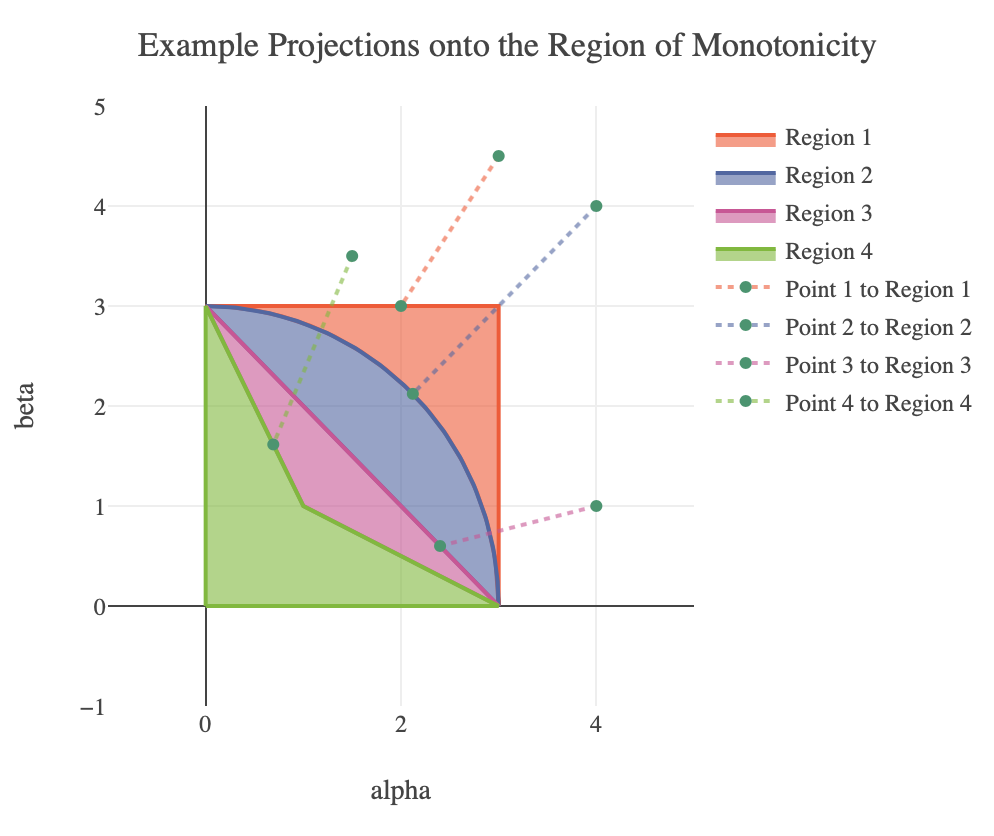
\includegraphics[width=0.50\textwidth]{demo_projection}
%%   \caption{These are the projection mechanisms that make a cubic polynomial piece monotone.}\label{fig:projection}
%% \end{figure}

%% The ability to interpolate or regress a function with continuous value and derivatives has proven fundamentally useful. In many applications, there are known shapes or characteristics that are expected of approximations. For example, a cumulative distribution function in statistics cannot decrease, the entropy of a closed thermodynamic system can never increase, an electric motor should not suddenly change direction when slowing down or speeding up. In each of these cases it is important that any constructed spline approximation is monotone.


Many domains of science rely on smooth approximations to real-valued functions over a closed interval. Piecewise polynomial functions (splines) provide the smooth approximations for animation in graphics \cite{herman2015techniques,quint2003scalable}, aesthetic structural support in architecture \cite{brennan2019measure}, efficient aerodynamic surfaces in automotive and aerospace engineering \cite{brennan2019measure}, prolonged effective operation of electric motors \shortcite{berglund2009planning}, and accurate nonparametric approximations in statistics \cite{knott2012interpolating}. While polynomial interpolants and regressors apply broadly, splines are often a good choice because they can approximate globally complex functions while minimizing the local complexity of an approximation.

It is often the case that the true underlying function or phenomenon being modeled has known properties e.g., convexity, positivity, various levels of continuity, or monotonicity. Given a reasonable amount of data, it quickly becomes difficult to achieve desirable properties in a single polynomial function. In general, the maintenance of function properties through interpolation/regression is referred to as \textit{shape preserving} \cite{fritsch1980monotone,gregory1985shape}. The specific shapes this work will achieve in approximations are monotonicity and $C^2$ continuity. These properties are chiefly important to the approximation of cumulative distribution functions and subsequently the effective generation of random numbers from a specified distribution.

In statistics especially, the construction of a monotone interpolating spline that is $C^2$ continuous is meaningfully useful \cite{ramsay1988monotone}. A function with these properties could approximate a cumulative distribution function to a high level of accuracy with relatively few intervals. A twice continuously differentiable approximation to a cumulative distribution function (CDF) would also produce a corresponding probability density function (PDF) that is continuously differentiable, which is a property many standard parametric distributions maintain.

The currently available software for monotone piecewise polynomial interpolation includes quadratic \cite{he1998monotone}, cubic \cite{fritsch1980monotone}, and (with limited application) quartic \cite{wang2004rational,piah2011improved,yao2018unconditionally} cases. In addition, a statistical method for bootstrapping the construction of an arbitrarily smooth monotone fit exists \cite{leitenstorfer2006generalized}, but the method does not take advantage of known analytic properties related to quintic polynomials. Theory has been provided for the quintic case \cite{ulrich1994positivity,hess1994positive}, however this theory has not yet been used to construct a monotone quintic spline interpolation routine. Recent work suggests that the lack of quintic software may be due to a general unawareness of the theory \shortcite{xie2018semiparametric}.

\begin{figure}
  \centering
  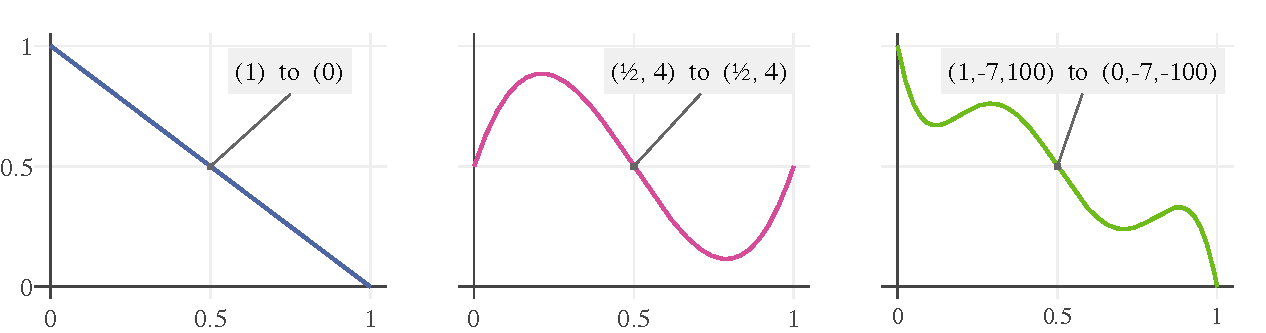
\includegraphics[width=.9\textwidth]{spline_demonstration}
  \caption{Example polynomials that interpolate function values at the ends of the interval $[0,1]$. The first only interpolates the function values $g_2(0) = 1$ and $g_2(1) = 0$, making it the order two polynomial $g_2(x) = 1 - x$. For the second plot $g_4(x) = 8x^3 - 12x^2 + 4x + 1/2$, which is order four and interpolates the values $g_4(0) = 1/2$, $g_4'(0) = 4$, $g_4(1) = 1/2$, $g_4'(1) = 4$. Finally the third plot shows the order six polynomial $g_6(x) = - 64x^5 + 160x^4 - 140x^3 + 50x^2 - 7x + 1$ interpolating the function values $g_6(0) = 1$, $g_6'(0) = -7$, $g_6''(0) = 100$, $g_6(1) = 0$, $g_6'(1) = -7$, $g_6''(1) = -100$. Notice that interpolating the same fixed number of function values at each endpoint will always result in an even order interpolating polynomial.
  }\label{fig:spline_demonstration}
\end{figure}

The importance of piecewise quintic interpolation over lower order approximations can be simply demonstrated. In general, the order of a polynomial determines the number of function values it can interpolate, and the growth rate of error away from the interpolated function values. As demonstrated in Figure \ref{fig:spline_demonstration}, it can be seen that matching a value at either end of the interval requires an order two (linear) approximation and each additional derivative at the ends of the interval raises the necessary polynomial order by two. Hence, only even order (odd degree) interpolating splines are broadly applicable. The body of this work is composed of a novel algorithm for enforcing monotonicity on quintic polynomial pieces, then extending that solution to work on quintic splines.

%% Software exists that does monotone piecewise quintic regression \cite{}, but the available routines do not computationally take advantage of the quintic monotonicity theory. ???

The major contribution of this work is an algorithm for constructing monotone quintic interpolating splines that utilizes existing quintic monotonicity theory. The remainder of this paper is structured as follows: Section \ref{sec:monotone-cubic} summarizes the existing monotone cubic spline interpolation methodology, Section \ref{sec:monotone-quintic} presents an algorithm for constructing monotone quintic spline interpolants, Section \ref{sec:results} offers experiments and results with cubic and quintic methods, Sections \ref{sec:discussion} and \ref{sec:conclusion} discuss results and conclude.


\subsection{Computing a Monotone Cubic Interpolant}
\label{sec:monotone-cubic}

The current state-of-the-art monotone interpolating spline with a mathematical software implementation is piecewise cubic, continuously differentiable, and was first proposed in \cite{fritsch1980monotone} then expanded upon in \cite{carlson1985monotone}. Let $\pi: x_0 = k_1 < k_2 < \cdots < k_n = x_1$ be a partition of the interval $[x_0,x_1]$. Let $f: \mathbb{R} \rightarrow \mathbb{R}$ be $C^2$, and $\bigl\{f(k_i)\bigr\}_{i=1}^n$ and $\bigl\{\Delta_i\bigr\}_{i=1}^n$ be given sets of function and derivative values at the partition points for a monotone function $f$. Either $f(k_i) \leq f(k_{i+1})$, $i=1$, $\ldots$, $n-1$, and $\Delta_i\ge0$, $i=1$, $\ldots$, $n$, or $f(k_i) \geq f(k_{i+1})$, $i=1$, $\ldots$, $n-1$, and $\Delta_i\le0$, $i=1$, $\ldots$, $n$. Let $\hat f$ be a piecewise cubic polynomial defined in each subinterval $I_i = [k_i, k_{i+1}]$ by
\begin{align*}
h_i &= k_{i+1} - k_{i}, \quad
u(t) = 3t^2 - 2t^3, \quad
p(t) = t^3 - t^2,\\
\hat f(x) &= f(k_i) u\big((k_{i+1} - x) / h_i\big) +
f(k_{i+1}) u\big((x - k_i) / h_i\big) \\
&{} - h_i\Delta_i p\big((k_{i+1}-x)/h_i\big) + h_i\Delta_{i+1}
p\big((x-k_i)/h_i\big).
\end{align*}
Notice that a trivially monotone spline results when $\Delta_i = 0$, for $i = 1$, $\ldots$, $n$. However, such a spline has too many \textit{wiggles} for most applications. \citeN{carlson1985monotone} show that simple conditions on the derivative values can guarantee monotonicity, and that these conditions can be enforced in a way that ensures modifications on one interval will not break the monotonicity of cubic polynomials over any neighboring intervals. If $f(k_i) = f(k_{i+1})$, take $\Delta_i = \Delta_{i+1} =0$ and $\alpha =\beta =1$, otherwise let $\alpha = \big(\Delta_i (k_{i+1}-k_i)\big) / \big(f(k_{i+1}) - f(k_i)\big)$ and $\beta = \big(\Delta_{i+1}(k_{i+1}-k_i)\big) / \big(f(k_{i+1}) - f(k_i)\big)$. Monotonicity of a cubic polynomial over a subinterval can be maintained by ensuring that $\alpha$ and $\beta$ reside in any of the regions depicted in Figure \ref{fig:projection}.

\begin{figure}
  \centering
  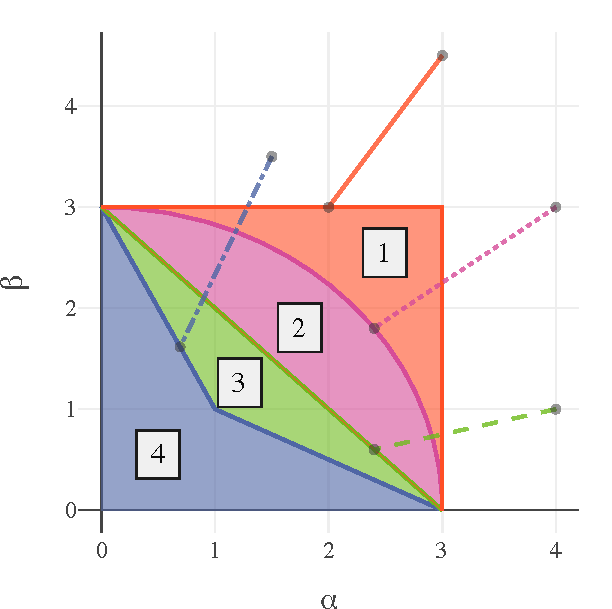
\includegraphics[width=0.40\textwidth]{cubic_projection_demonstration}
  \caption{These are the feasible regions of monotonicity for cubic splines and the projections that make a cubic polynomial piece monotone. The regions themselves are numbered 1--4 corresponding to their original description in Fritsch and Carlson (1980). One point is projected onto each region as a demonstration.}\label{fig:projection}
\end{figure}

The actual region of monotonicity for a cubic polynomial is larger, but projection of $(\alpha, \beta)$ into one of these regions ensures that monotonicity will be achieved and not violated for neighboring regions. The user must decide which region is most appropriate for the projections based on the application, Fritsch and Carlson recommend using Region 2.

While the cubic monotonicity case affords such a concise solution, the region of monotonicity is not so simple in the quintic case. In the next section, an algorithm for performing a projection similar to those for cubic polynomials is proposed.

\section{Monotone Quintic Interpolation}
\label{sec:monotone-quintic}

The following section is composed of three algorithms that together are used to construct a monotone quintic spline interpolant. Without loss of generality, the algorithms will only consider the monotone increasing (nondecreasing) case. The monotone decreasing case is handled similarly. Algorithm \ref{alg:check-monotone} checks monotonicity,
Algorithm \ref{alg:make-monotone} enforces monotonicity on an order six
polynomial piece of the quintic spline, and Algorithm
\ref{alg:monotone-spline} uses the previous two algorithms to enforce
monotonicity for the entire quintic spline.


In pseudocode, a function \texttt{binary\_search($g,$ $a,$ $b$)} is used, where $a,b\in S\subset \mathbb{R}^p$ for convex $S$, $g: S \rightarrow \{$\texttt{FALSE}, \texttt{TRUE}$\}$ is a right continuous Boolean function, $g(b) = \hbox{\texttt{TRUE}}$, and for $\mu \in [0,1]$, $g\big((1-\mu)a + \mu b\big) =\hbox{\texttt{TRUE}} \Longrightarrow g\big((1-\nu)a + \nu b\big) =\hbox{\texttt{TRUE}}$ for $\mu \le \nu\le1$. The search returns $\big((1-c)a + c b\big)$ for the smallest $c \in [0,1]$ such that $g\big((1-c)a + c b\big) = \hbox{\texttt{TRUE}}$.

These algorithms make use of first and second derivatives of the approximated function where $D$ denotes the differentiation operator. In the case that the first and second derivative information is not provided along with function values, the derivatives are estimated with finite differences of the function values. The final quintic spline is represented as a piecewise polynomial using the Newton form for each polynomial piece, and ultimately converted to a $B$-spline representation for evaluation.

\algorithm
    {is\_monotone$\big(x_0, x_1, f \big)$}
    {where $x_0$, $x_1 \in \mathbb{R}$, $x_0 < x_1$, and $f$ is an order six polynomial defined by $f(x_0)$, $Df(x_0)$, $D^2f(x_0)$, $f(x_1)$,
  $Df(x_1)$, $D^2f(x_1)$. Returns \texttt{TRUE} if $f$ is monotone increasing on $[x_0,x_1]$.}
    {\label{alg:check-monotone}
  \item if $\big(f(x_0) = f(x_1)\big)$ and not $\big( 0 = Df(x_0) = Df(x_1) = D^2f(x_0) = D^2f(x_1) \big)$
    \indented{return FALSE}
    end if
  \item if $\big(Df(x_0) < 0$ or $Df(x_1) < 0\big)$
    \indented{return FALSE}
    end if
    \comment{The necessity of these first two steps follows directly from the fact that $f$ is $C^2$. The next case is in accordance with a simplified condition for quintic monotonicity that reduces to one of cubic positivity studied in \citeN{schmidt1988positivity}, where $\alpha$, $\beta$, $\gamma$, and $\delta$ are defined in terms of values and derivatives of $f$ at $x_0$ and $x_1$. Step \ref{alg1-alpha} checks for the necessary condition that $\alpha \ge 0$, Step \ref{alg1-beta} checks $\beta \geq \alpha$, and Step \ref{alg1-gamma} checks $\gamma \geq \delta$, all from \citeN{schmidt1988positivity}. If all necessary conditions are met, then the order six piece is monotone and Step \ref{alg1-simplified-true} concludes this check.}
  \item if $\big(Df(x_0) = 0$ or $Df(x_1) = 0\big)$
  \item \indented{$w := x_0 - x_1$\\$v := f(x_0) - f(x_1)$}
  \item \indented{if $\big(D^2f(x_1) > {-4}Df(x_1) / w \big)$ return FALSE}
    \label{alg1-alpha}
  \item \indented{if $\big(D^2f(x_1) < (3w D^2f(x_0) - 24 Df(x_0) - 32
    Df(x_1) + 60v/w) / (5w) \big)$ return FALSE} \label{alg1-beta}
  \item \indented{if $\big(D^2f(x_0) < 3 Df(x_0) / w \big)$ return FALSE}
    \label{alg1-gamma}
  \item \indented{return TRUE} \label{alg1-simplified-true}
    end if
    \comment{The following code considers the remaining case where $Df(x_0) \neq 0$ and $Df(x_1) \neq 0$.}
  \item $\displaystyle A := Df(x_0)\frac{x_1 - x_0}{f(x_1) - f(x_0)}$
    \\ $\displaystyle B := Df(x_1) \frac{x_1 - x_0}{f(x_1) - f(x_0)}$
    \comment{The variables $A$ and $B$ correspond directly to the theoretical foundation for positive quartic polynomials established in \citeN{ulrich1994positivity}, first defined after Equation (18).}
  \item $\displaystyle \gamma_0 := 4 \frac{Df(x_0)}{Df(x_1)} (B/A)^{3/4}$
    \\ $\displaystyle \gamma_1 := \frac{x_1 - x_0}{Df(x_1)} (B/A)^{3/4}$
    \\ $\alpha_0 := 4 (B/A)^{1/4}$
    \\ $\displaystyle \alpha_1 := -\frac{x_1 - x_0}{Df(x_1)} (B/A)^{1/4}$
    \\ $\displaystyle \beta_0 := 30 - \frac{12 \big(Df(x_0) + Df(x_1)\big) (x_1 - x_0)}{\big(f(x_1) - f(x_0)\big) \sqrt{A}\sqrt{B}}$
    \\ $\displaystyle \beta_1 := \frac{-3 (x_1 - x_0)^2}{2 \big(f(x_1) - f(x_0)\big) \sqrt{A} \sqrt{B}} $ \label{alg1-linearized-abg}
    \comment{The $\gamma$, $\alpha$, and $\beta$ terms with subscripts $0$ and $1$ are algebraic reductions of the simplified conditions for satisfying Theorem 2 in Equation (16) of \citeN{ulrich1994positivity}. These terms with subscripts $0$ and $1$ make the computation of $\alpha$, $\beta$, and $\gamma$ functions of the second derivative terms, as seen in Step \ref{alg1-abg} below.}
  \item $\gamma := \gamma_0 + \gamma_1 D^2f(x_0)$
    \\ $\alpha := \alpha_0 + \alpha_1 D^2f(x_1)$
    \\ $\beta := \beta_0 + \beta_1 \big(D^2f(x_0) - D^2f(x_1)\big)$
    \label{alg1-abg}
  \item if $(\beta \leq 6)$ return $\big(\alpha > - (\beta + 2) / 2\big)$
    \\ else $\qquad$ return $\big(\gamma > -2 \sqrt{\beta - 2}\big)$
    \\ end if \label{alg1-last}
}
%% ----------------------------------------------------------------------

The reason for structuring the $\alpha$, $\beta$, and $\gamma$ computations in terms of the second derivative of $f$ (seen in Step \ref{alg1-abg} of Algorithm \ref{alg:check-monotone}) will become more apparent later. The next problem to consider is that of making a nonmonotone order six polynomial piece into a monotone one by modifying its first and second derivative values at the ends of an interval. Note that the actual value of the function at the ends of the interval is not modified, as the resulting polynomial needs to interpolate.

%% ----------------------------------------------------------------------
\algorithm
    {make\_monotone$\big (x_0$,$x_1$,$f \big)$}
    {where $x_0,\ x_1 \in \mathbb{R}$, $x_0 < x_1$, and $f$ is an order six polynomial defined by $f(x_0)$, $Df(x_0)$, $D^2f(x_0)$, $f(x_1)$, $Df(x_1)$, $D^2f(x_1)$. Returns $f$ monotone on $[x_0,x_1]$.}
    {\label{alg:make-monotone}
    \item if $\big(f(x_1) = f(x_0)\big)$
      \indented{$Df(x_0) := Df(x_1) := D^2f(x_0) := D^2f(x_1) := 0$}
      \indented{return}
      end if
    \item $Df(x_0) :=\ $median$\displaystyle \bigg(0,\ Df(x_0),\ 14 \frac{f(x_1) - f(x_0)}{x_1 - x_0} \bigg)$
      \\ $Df(x_1) :=\ $median$\displaystyle \bigg(0,\ Df(x_1),\ 14 \frac{f(x_1) - f(x_0)}{x_1 - x_0}\bigg)$ \label{alg2-init-df}
      \comment{The selection of values in Step \ref{alg2-init-df} for $Df(x_0)$ and $Df(x_1)$ is suggested by \citeN{ulrich1994positivity} and also by \citeN{huynh1993accurate}. These rules quickly enforce upper and lower bounds on derivative values to ensure quintic monotonicity is obtainable.}
      \comment{The next case that will be covered is in accordance with a simplified condition for quintic monotonicity that reduces to one of cubic positivity studied in \citeN{schmidt1988positivity}, where $\alpha$, $\beta$, $\gamma$, and $\delta$ are defined in terms of values and derivatives of $f$ at $x_0$ and $x_1$. Steps \ref{alg2-dx-conditions} and \ref{alg2-rescale-dx} ensure that the following bounds on $D^2f(x_0)$ are compatible while Step \ref{alg2-ddx0-upper} ensures that the conditions on $D^2f(x_1)$ are compatible. To conclude the simplified case, Step \ref{alg2-gamma} first enforces $\gamma \geq \delta$, then Steps \ref{alg2-alpha} and \ref{alg2-beta} enforce $\alpha \geq 0$ and $\beta \geq \alpha$ respectively. Combined, these three conditions derived from Equation (2.18) in \citeN{schmidt1988positivity} guarantee monotonicity of this polynomial piece.}
    \item if $\big(Df(x_0) = 0$ or $Df(x_1) = 0\big)$
    \item \indented{$w := x_0 - x_1$\\$v := f(x_0) - f(x_1)$}
    \item \indented{if $\big(5 Df(x_0) + 4Df(x_1) > 20v / w)$} \label{alg2-dx-conditions}
    \item \indented{\indented{$Df(x_0) := Df(x_0) \text{ max}\displaystyle \bigg(0, \frac{20v}{w \big(5 Df(x_0) + 4 Df(x_1)\big)}\bigg) $}}
      \indented{\indented{$Df(x_1) := Df(x_1) \text{ max}\displaystyle \bigg(0, \frac{20v}{w \big(5 Df(x_0) + 4 Df(x_1)\big)}\bigg) $}} \label{alg2-rescale-dx}
      \indented{end if}
    \item \indented{$D^2f(x_0) :=\ $min$\displaystyle \bigg(D^2f(x_0), \frac{4 (2 Df(x_0)+Df(x_1))+20 v/w}{w} \bigg)$} \label{alg2-ddx0-upper}
    \item  \indented{$D^2f(x_0) :=\ $max$\big(D^2f(x_0), 3 Df(x_0) / w \big)$} \label{alg2-gamma}
    \item \indented{$D^2f(x_1) :=\ $min$\big(D^2f(x_1), {-4}Df(x_1) / w \big)$} \label{alg2-alpha}
    \item  \indented{$D^2f(x_1) :=\ $max$\displaystyle \bigg(D^2f(x_1), \frac{3w D^2f(x_0) - 24 Df(x_0) - 32 Df(x_1) + 60v/w}{5w} \bigg)$} \label{alg2-beta}
      \indented{return}
      end if
      \comment{The following code considers the case where $Df(x_0) \neq 0$ and $Df(x_1) \neq 0$.}
    \item $\displaystyle A := Df(x_0)\frac{x_1 - x_0}{f(x_1) - f(x_0)}$
      \\ $\displaystyle B := Df(x_1) \frac{x_1 - x_0}{f(x_1) - f(x_0)}$
    \item if $\big($max$(A,B) > 6\big)$
      \indented{$Df(x_0) := 6 Df(x_0) \big/ $max$(A,B)$}
      \indented{$Df(x_1) := 6 Df(x_1) \big/ $max$(A,B)$}
      end if
      \comment{This ensures that $(A,B)$ remains within a viable region of monotonicity (satisfying Theorem 4, seen in Fig. 6 of \citeN{ulrich1994positivity}).}
    \item $\eta := \big(D^2f(x_0), D^2f(x_1)\big)$
      \\ $\displaystyle \eta_0 := \left({-\frac{\sqrt{A}}{4}}\big(7\sqrt{A} + 3\sqrt{B}\big),\ \frac{\sqrt{B}}{4}\big(3\sqrt{A} + 7\sqrt{B}\big) \right)$
    \item $\bigl(D^2f(x_0)$, $D^2f(x_1)\bigr) :=$ binary\_search$\bigl(g,
       \eta,\eta_0\bigr)$
      \comment{Here $g(z) =$\texttt{ is\_monotone}$(x_0,x_1,f)$ where $x_0$, $x_1$, $f(x_0)$, $f(x_1)$, $Df(x_0)$, $Df(x_1)$ are fixed, and the variable $z=\bigl(D^2f(x_0)$,$D^2f(x_1)\bigr)$. This binary search identifies feasible values of $D^2f(x_0)$ and $D^2f(x_1)$ that are nearest to the current values $\eta$. This search is valid because $\eta_0$ is guaranteed to produce a monotone function, which can be seen in Equation (23) of \citeN{ulrich1994positivity}.}
    return
}
%% ----------------------------------------------------------------------


Notice that both Algorithms \ref{alg:check-monotone} and \ref{alg:make-monotone} have $\mathcal{O}(1)$ runtime assuming a fixed level of precision is chosen beforehand. A constant number of operations are needed for verifying monotonicity (Algorithm \ref{alg:check-monotone}), while a constant set of operations and a single binary search are performed for enforcing monotonicity (Algorithm \ref{alg:make-monotone}). The search requires a fixed number of steps to achieve any predetermined relative precision, since its accuracy is predetermined and not a function of the problem at hand. Also note that an efficient implementation of Algorithm \ref{alg:make-monotone} only needs to recalculate Steps \ref{alg1-abg} and \ref{alg1-last} of Algorithm \ref{alg:check-monotone} during the binary search. Next, an algorithm for constructing a monotone quintic spline interpolant is presented.

%% ----------------------------------------------------------------------

\algorithm
    {monotone\_spline$\big((k_1$, $\ldots$, $k_n)$, $f$, $s\big)$}
    {where $(k_1$, $\ldots$, $k_n)$ is an increasing sequence of real numbers, $f$ is an order six piecewise polynomial with breakpoints $k_1$, $\ldots$, $k_n$ defined by the data $\bigl\{f(k_i)\bigr\}_{i=1}^n$, $\bigl\{Df(k_i)\bigr\}_{i=1}^n$, $\bigl\{D^2f(k_i)\bigr\}_{i=1}^n$, and $s > 1$ is an integer shrink factor.}
    {\label{alg:monotone-spline}
    \item create queue
      \\ create changed$(1$, $\ldots$, $n) := $ FALSE
      \\ create step\_size$(1$, $\ldots$, $n) := \bigl(Df(k_1)/s$, $\ldots$, $Df(k_n)/s\bigr)$ \label{step:create}
      \comment{The three variables defined in Step \ref{step:create} are used to ensure the eventual achievement of monotonicity. The \texttt{queue} is a standard first in first out (FIFO) queue with \texttt{enqueue} and \texttt{dequeue} operations. The array \texttt{changed} contains Booleans describing whether or not a breakpoint belongs to an interval that has been modified to enforce monotonicity. The \texttt{step\_size} array contains the real-valued derivative decrement step sizes to use in the search for a valid monotone spline.}
    \item for $i := 1$, $\ldots$, $n-1$
      \indented{enqueue $\bigl((k_i, k_{i+1})\bigr)$}
      end for
      \comment{Initially, all intervals must be checked for monotonicity. The following loop will continue until all intervals are verified as monotone without need for modification.}
    \item while $($size$($queue$) > 0)$
    \item \indented{$(k_j$, $k_{j+1}) := $ dequeue}
    \item \indented{if $\big($not is\_monotone$(k_j$, $k_{j+1}$, $f)\big)$}
    \item \indented{\indented{if $\big($changed$(j)\big) \qquad \ Df(k_j) := Df(k_j) -{}$step\_size$(j)$}}
      \indented{\indented{if $\big($changed$(j+1)\big) \quad Df(k_{j+1}) := Df(k_{j+1}) -{}$step\_size$(j+1)$}}
      \indented{\indented{\comment{If a breakpoint belongs to an interval that has been previously modified, then the enforced monotonicity conditions on the second derivatives of adjacent intervals must contradict one another. In turn, the involved first derivatives are decreased towards zero by a predetermined step size.}}}
    \item \indented{\indented{make\_monotone$(k_j,\ k_{j+1},\ f)$}}
    \item \indented{\indented{changed$(j) :=$ TRUE}}
      \indented{\indented{changed$(j+1) :=$ TRUE}} \label{step:changed}
    \item \indented{\indented{if $\big(j > 1$ and $(k_{j-1}, k_j) \not\in$ queue$\big)$ enqueue $\bigl((k_{j-1}, k_j)\bigr)$}}
      \indented{\indented{enqueue $\bigl((k_j, k_{j+1})\bigr)$}}
      \indented{\indented{if $\big(j+1 < n$ and $(k_{j+1}, k_{j+2}) \not\in$ queue$\big)$ enqueue $\bigl((k_{j+1}, k_{j+2})\bigr)$}} \label{step:requeue}
      \indented{\indented{\comment{Step \ref{step:changed} records the endpoints of the current interval as having been changed, while \ref{step:requeue} adds adjacent intervals to \texttt{queue} that may have inadvertently been made nonmonotone by the changes to the present interval.}}}      
      \indented{end if}
      end while
}
%% ----------------------------------------------------------------------

It is mentioned in \citeN{ulrich1994positivity} that for sufficiently small $Df(k_i)$ and $Df(k_{i+1})$ the admissible solution interval of second derivative values becomes arbitrarily large. It can also be seen that decreasing the assigned derivative values towards zero will eventually cause Steps \ref{alg1-alpha} through \ref{alg1-gamma} of Algorithm \ref{alg:check-monotone} to all fail, resulting in Step \ref{alg1-simplified-true} returning \texttt{TRUE}.

If successive monotonicity fixes are required for all intervals, the worst case runtime of Algorithm \ref{alg:monotone-spline} is $\mathcal{O}(s n)$ for $n$ breakpoints and shrink factor $s$. In practice this worst case has been observed to be unlikely.

\section{Experimental Results}
\label{sec:results}

Given the increased order of approximation, it is naturally expected that some accuracy benefit could be gained by using a quintic spline over a cubic spline. Experiments 1 and 2 below test some accuracy differences between monotone cubic and quintic splines. Experiment 3 analyzes the number of operations performed by Algorithm \ref{alg:monotone-spline} with increasingly large samples of monotone data.

\subsection{Approximating a Trigonometric Function}

For this experiment, the function $\sin(x) + x$ is considered over the interval $[0,(5/2)\pi]$ as seen in Figure \ref{fig:cubic_quintic_sin}. Given an increasing number of points, the maximum error of cubic and quintic approximations is shown in Figure \ref{fig:experiment_1}. The quintic approximation consistently has a maximum error that is roughly half that of the cubic approximation, given the same number of points. There is an increase in the error gap between the two approximations as more points are added. The quintic spline requires only $700$ points to approximate the function to the same accuracy achieved by the cubic with $1000$ points.

\begin{figure}[h]
  \centering
  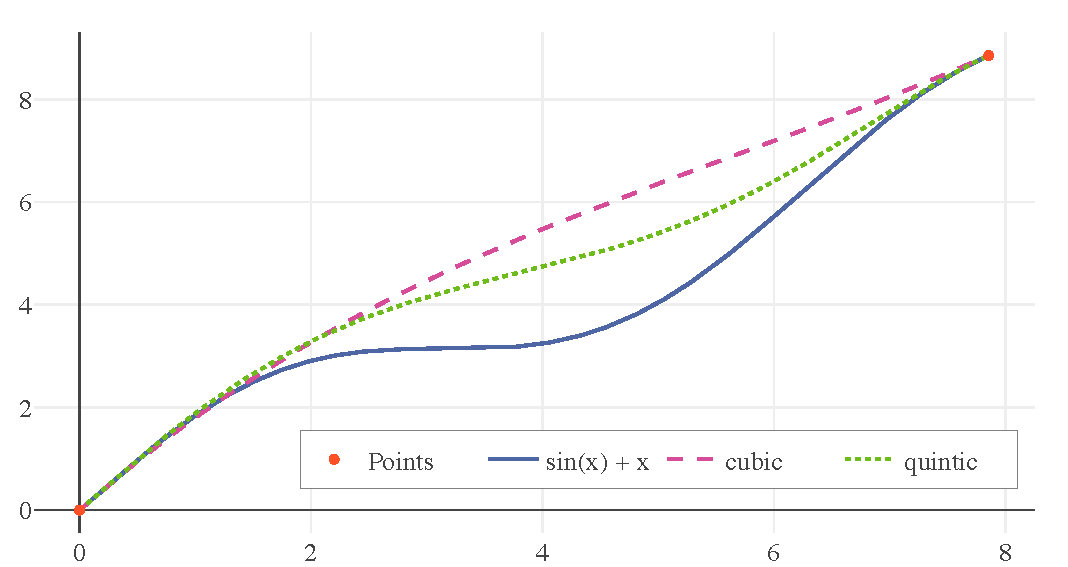
\includegraphics[width=.7\textwidth]{cubic-quintic-sin}
  \caption{Depicted above are the monotone cubic and quintic spline interpolants of the function $\sin(x) + x$ over the points $[0, (5/2) \pi]$.  Notice that the maximum error of the cubic interpolant is larger, because it only captures first derivative information at the points. The quintic interpolant captures both first and second derivative information at the points.}
  \label{fig:cubic_quintic_sin}
\end{figure}

\begin{figure}
  \centering
  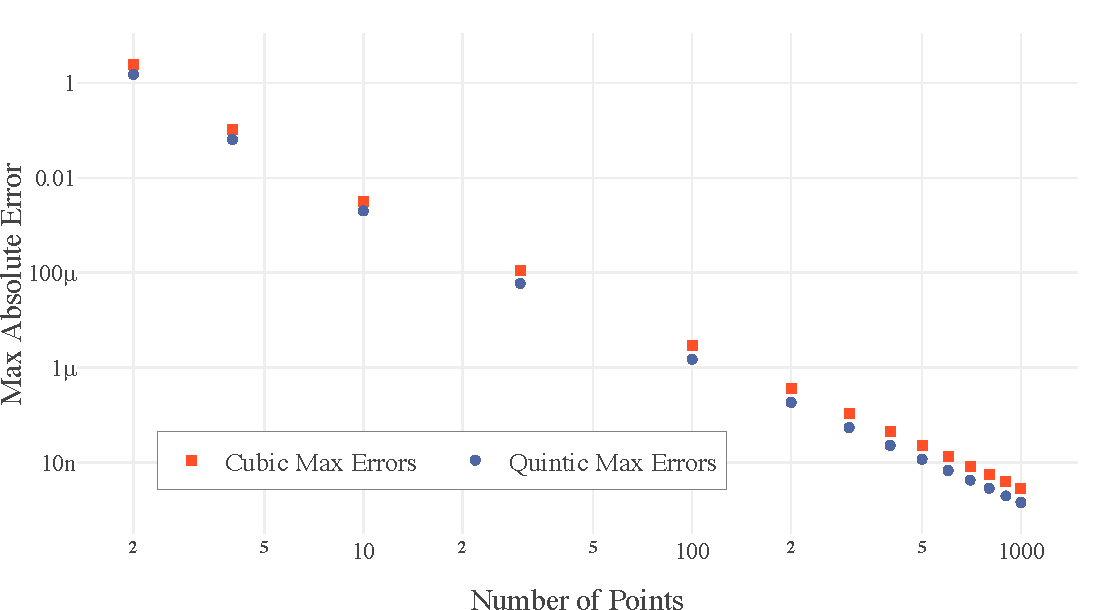
\includegraphics[width=.7\textwidth]{experiment_1_errors}
  \caption{The error in the quintic and cubic approximations of $\sin(x) + x$ with increasing number of points. Both axes are log scaled, where $\mu$ means $\times 10^{-6}$ and n means $\times 10^{-9}$ on the vertical axis. The quintic approximation generally provides an approximation with about half of the maximum error of the cubic approximation, while the relative gap between grows with increasing number of points. In order to achieve the same absolute error the quintic spline requires ten fewer points at max error $10^{-4}$, thirty fewer points at max error $10^{-6}$, and $300$ fewer points at max error $10^{-8}$.}
  \label{fig:experiment_1}
\end{figure}


\subsection{Random Number Generation}

Consider the cumulative distribution function (CDF) defined by a mixture of three Gaussian distributions and visualized in Figure \ref{fig:experiment_2_distribution}. The distributions have weights $(.3, .6, .1)$, means $(.2, .45, .85)$ and standard deviations $(.05, .08, .03)$. $200$ random samples are generated from this distribution with both cubic and quintic approximations from four points, and over $100$ trials the resulting spread of empirical distribution functions (EDFs) are visualized in Figure \ref{fig:experiment_2_results}.

While an increased number of points could be used to decrease the error in either approximation, the purpose of this experiment is to demonstrate the effect approximation error has on random number generation. The errors in the CDFs are magnified by the variance involved in randomly sampling from a distribution. As a result, while the cubic and quintic spline approximations have similar maximum error, the cubic distribution is significantly distorted around the first and second modes.

\begin{figure}
  \centering
  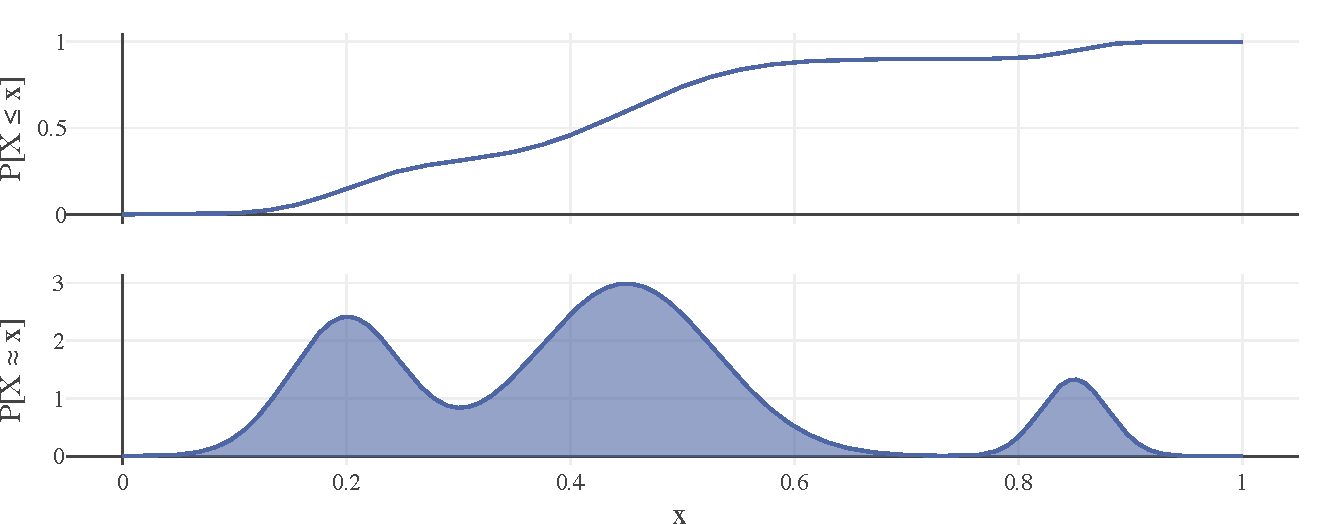
\includegraphics[width=.8\textwidth]{experiment_2_distribution}
  \caption{The cumulative distribution function (top) and probability density function (bottom) for the Gaussian mixture distribution in Experiment 2. The distributions have weights $(.3, .6, .1)$, means $(.2, .45, .85)$ and standard deviations $(.05, .08, .03)$. Random samples are generated from this mixture distribution by evaluating the inverse of the CDF at random numbers uniformly distributed in the range $[0,1]$.}
  \label{fig:experiment_2_distribution}
\end{figure}

\begin{figure}
  \centering
  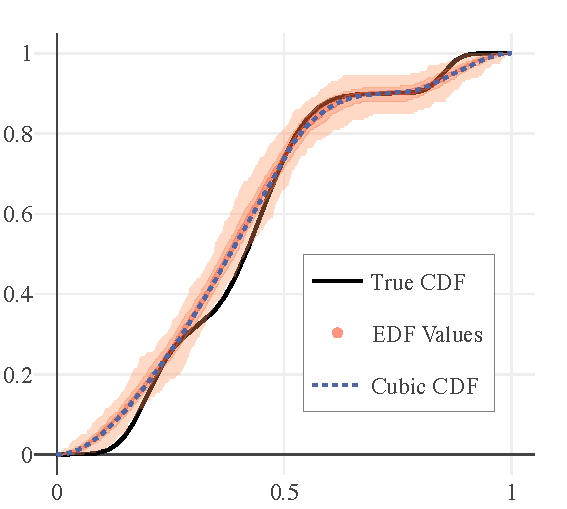
\includegraphics[width=.4\textwidth]{experiment_2_cubic_dist}
  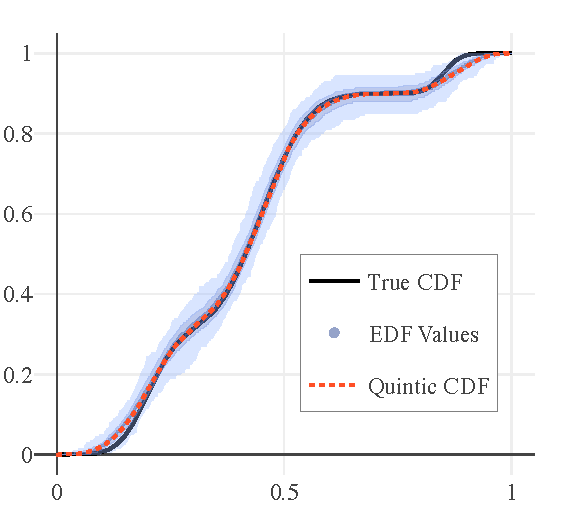
\includegraphics[width=.4\textwidth]{experiment_2_quintic_dist}
  \caption{Both cubic and quintic splines are used to approximate the CDF of a Gaussian mixture distribution with three components. Four CDF points are used to build the approximation, $200$ random samples are generated with the approximate CDFs over $100$ trials. The resulting cloud of empirical distribution function (EDF) values is seen above. The maximum approximation error in the CDFs are similar, $.08$ for the cubic and $.05$ for the quintic. However, the maximum EDF differences observed are doubled by the variance of random samples, $.15$ for the cubic and $.1$ for the quintic.}
  \label{fig:experiment_2_results}
\end{figure}

%% - generate large sets of random monotone data, show Table of number
%%   of metrics growing with increasing number of points

%% - show visual of the \textit{error} 

\subsection{Random Monotone Data}

This experiment studies the number of times the algorithms \texttt{is\_monotone} and \texttt{make\_monotone} are executed for increasingly large sequences of random monotone data. The minimum, median, and maximum number of times that Algorithms \ref{alg:check-monotone} and \ref{alg:make-monotone} are executed is recorded, as well as the number of steps taken in all calls to \texttt{binary\_search}. The number of calls and steps grows linearly with $n$ as expected, requiring roughly one call to \texttt{make\_monotone} and $20$ binary search steps to create a monotone piece. Some (less common) problems require an average of three calls to \texttt{make\_monotone} per interval.

\begin{table}
  \centering
  \begin{tabular}{c|c c c|c c c|c c c}
    \hline
    \multirow{2}{*}{$n$}
      & \multicolumn{3}{c|}{Checks} & \multicolumn{3}{c}{Fixes} & \multicolumn{3}{|c}{Search Steps} \\
      & min & median & max & min & median & max & min & median & max \\
    \hline
    5 & 4 & 6 & 274 & 0 & 1 & 154 & 3 & 31 & 2006\\
    25 & 28 & 47 & 378 & 2 & 14 & 225 & 80 & 348 & 3742\\
    50 & 61 & 124 & 484 & 6 & 40 & 238 & 217 & 851 & 4445\\
    75 & 102 & 216 & 842 & 14 & 74 & 411 & 463 & 1491 & 6333\\
    100 & 142 & 306 & 776 & 21 & 107 & 380 & 629 & 2140 & 7414\\
    \hline
  \end{tabular}
  \caption{The minimum, median, and maximum number of checks, fixes, and binary search steps required in the execution of \texttt{make\_spline} for increasing size sequences, $n$, over $100$ randomly generated sets of monotone data. Notice the maximum for each counter is often significantly greater than the minimum and median, because the distribution of each counter is skewed right.}
  \label{table:e3_results}
\end{table}

\section{Discussion}
\label{sec:discussion}

The monotone quintic spline interpolant provides a distinct increase in accuracy over the monotone cubic variant. The computational complexity of this algorithm is identical to the existing cubic method and the cost of evaluating the spline after construction is unchanged. While the number of computations required per interval has increased, the number of points required to achieve the same level of accuracy has decreased. In the present state, the algorithm for enforcing monotonicity on a spline is not as trivially parallel as the cubic algorithm, however it can still be parallelized. The checks for monotonicity across all intervals are independent and the monotonicity adjustments could be computed independently and intelligently merged with minor changes to the serial algorithm.

Acknowledging that the algorithm for constructing a monotone quintic spline interpolant is slightly more expensive than the cubic case, gains in accuracy or decreased necessary number of points are often worth the computational effort. In practice the costs of spline interpolation are often dominated by evaluation rather than construction, and the increased accuracy is afforded for a negligible increase in computational cost.

\section{Conclusion and Future Work}
\label{sec:conclusion}

This paper proposes and tests an algorithm for constructing monotone quintic spline interpolants. Experiments demonstrate an improvement in approximation accuracy over monotone cubic spline interpolants, as expected based on theory. There are still open avenues of research going forward, such as an alternative sufficient condition for enforcing monotonicity or increased order monotone approximations. If the monotonicity conditions can be generalized to any order or made linear, the search for a monotone interpolating spline could potentially be formulated as a convex optimization problem. Finally, this work could be used to improve cumulative distribution function (CDF) estimates as well as predictive models that use CDFs.


\section*{Acknowledgments}
This work was supported by the National Science Foundation Grants CNS-1565314 and CNS-1838271.

% Please don't change the bibliographystyle style
\bibliographystyle{scsproc}
% AUTHOR: Include your bib file here
\bibliography{paper}


\section*{Author Biographies}

\textbf{\uppercase{THOMAS C. H. LUX}} is a Ph.D. candidate in computer
science at Virginia Polytechnic Institute and State University
(VPI\&SU) studying under Dr. Layne Watson. His email address is
\email{tchlux@vt.edu}.

\textbf{\uppercase{Layne T. Watson}} (Ph.D., Michigan, 1974) has
interests in numerical analysis, mathematical programming,
bioinformatics, and data science.  He has been involved with the
organization of HPCS since 2000.

\textbf{\uppercase{Tyler H. Chang}} is a Ph.D. candidate at VPI\&SU
studying computer science under Dr. Layne Watson.

\textbf{\uppercase{Li Xu}} is a Ph.D. candidate at VPI\&SU studying
statistics under Dr. Yili Hong.

\textbf{\uppercase{Yueyao Wang}} is a Ph.D. candidate at VPI\&SU
studying statistics under Dr. Yili Hong.

\textbf{\uppercase{Yili Hong}} (Ph.D., Iowa State, 2009) is an
associate professor of Statistics at VPI\&SU.


%% \newpage

%% \appendix

%% \section{Author Checklist}
%% We strive for a consistent appearance in all papers published in the proceedings. If you used the template and styles within this author’s kit, then almost all of the requirements in this checklist will be automatically satisfied, and there is very little to check.

%% Please \textbf{print a hardcopy of your paper}, and go over your printed paper to make sure it adheres to the following requirements. \textit{Thank you!}

%% \begin{enumerate}
%% 	\item Abstract
%%   \begin{enumerate}
%% 	  \item 150 or fewer words.
%% 	  \item Provide 3-5 keywords (mandatory). This set of keywords will identify your paper in indices and databases.
%% 	\end{enumerate}
%% 	\item Paper Length
%%   \begin{enumerate}
%% 	  \item At least 5, but no more than 12 pages.
%% 	  \item Page size is letter size (8.5’’ x 11’’, or 216 mm x 279 mm).
%% 	\end{enumerate}
%% 	\item All text is in 11-Point Times New Roman except title, header and footer (default in this template).
%% 	\item Paper title is in 12-Point Times New Roman \textbf{BOLDFACE ALL CAPS} (default in this template).
%% 	\item The paper has been spellchecked using U.S. English. 
%% 	\item Spacing and Margins
%%   \begin{enumerate}
%% 	  \item Single spaced.
%% 	  \item Left and right margins are each 1 inch (default in this template).
%% 	  \item Top and bottom margins are according to the template.
%% 	  \item Title starts 1.25 inches from the top of the page (default in this template).
%% 	\end{enumerate}
%% 	\item Section Headings
%%   \begin{enumerate}
%% 	  \item Left justified and set in \textbf{BOLDFACE ALL CAPS} (default in this template).
%% 	  \item Numbered, except for the abstract, acknowledgments, references and author biographies.
%% 	  \item Subsection headings are set in \textbf{Boldface Headline Style} (default in this template).
%% 	\end{enumerate}
%% 	\item No footnotes or page numbers.
%% 	\item The copyright notice on the first page contains the name of the symposium or a track where you want to submit your paper, and the running head on subsequent pages is the surnames of all authors.
%% 	\item Multiple authors are formatted correctly.
%% 	\item Equations are centered and any equation numbers are in parentheses and right-justified (default).
%% 	\item Figures and Tables
%%   \begin{enumerate}
%% 	  \item All text in figures and tables is readable.
%% 	  \item Table captions appear above the table.
%% 	  \item Figure captions appear below the figure.
%% 	\end{enumerate}
%% 	\item Citations and References
%%   \begin{enumerate}
%% 	  \item Citations are by author and year, and are enclosed in parentheses, not brackets (default \BibTeX). 
%% 	  \item References are in the hangref style, and are listed alphabetically by the last names(s) of the author(s) (also default \BibTeX\ setting in this template). 
%% 	\end{enumerate}
%% 	\item Author biographies are one paragraph per author.
%% 	\item Hyperlinks
%%   \begin{enumerate}
%% 	  \item Be sure that hyperlinks will probably work in the future as well.
%% 	  \item Live hyperlinks are blue. Nonlive hyperlinks are black (default in this template).
%% 	\end{enumerate}
%% 	\item All fonts must be embedded in the resulting \texttt{.pdf}. If you use \texttt{pdflatex}, this should already be true--unless you included figures in the \texttt{.eps} or \texttt{.pdf} format which may introduce additional font dependencies. You can use the \texttt{pdffonts} command to see if all the fonts are embedded (the column ``emb'' should say yes for all rows). You can use GhostScript to force embed the fonts, like so: {\texttt{gs -dNOPAUSE -dBATCH -sDEVICE=pdfwrite -dEmbedAllFonts=true -sOutputFile=out.pdf -f in.pdf}} (in Windows, use \texttt{gswin32} or \texttt{gswin32c} to invoke GhostScript).
%% \end{enumerate}

%% After verifying that your paper meets these requirements, please go to the final submission page at conference website and submit your paper. Be sure to complete the transfer of copyright form and upload the \texttt{.pdf} receipt. \textit{Thank you for contributing to the SCS conferences!}

%% \section{Most Observed Mistakes}

%% The following list comprises \textbf{the most common sources of error} that had to be corrected by previous editors. Please make sure to go through the following list and check that your paper is formatted correctly:
%% \begin{enumerate}
%% 	\item	The paper is less than 5 or more than 12 pages long.
%% 	\item	Paper title and section titles are in \textbf{BOLD ALL CAPS}, subsections are \textbf{Bold and Capitalize the First Letter of Important Words}. Please use the templates.
%% 	\item	Paper is in A4 format, not letter format. Please use the required margins.
%% 	\item	The copyright notice is incorrect.
%% 	\item	The running heads are incorrect. Do not forget that the LastNameLastAuthor is preceded by ``, and ''.
%% 	\item	The citation format is incorrect. Use \BibTeX\ for citations and do not change the format used by the template.
%% 	\item	The biographies are missing. Do not forget the ``author biographies'' section.
%% 	\item	Figures or tables are not referenced in the text or have the incorrect caption format.
%% 	\item	The author section after the title is not formatted correctly, the number of organizations does not define the number of blocks, or the number of blocks does not define the layout.
%% 	\item In the heading on the title page, country names are in all capitals.
%% 	\item	Paragraphs are not indented.
%% 	\item Some fonts in the resulting \texttt{.pdf} are not embedded.
%% \end{enumerate}



\end{document}
